In order to evaluate the performance of our system we examined the percentage of frames 
correctly classified with our segmentation and with perfect segmentation. The perfect
segmentation and ground truth label for each frame were determined using the annotation
to the development data.

The percentage of frames correct given perfect segmentation gives a sense of how well the
classification stage of our system performs. Currently, given perfect segmentation,
our system correctly classifies 48\% of frames. 

The percentage of frames correct with segmentation determined by our system when compared to the other metric
gives a good sense of how segmentation effects classification. With our segmentation, the 
system correctly classified 25\% of frames.

The confusion matricies of classifier stages of the perfectly segmented events, as well as the events segmented using our algorithm can be seen in Figure \ref{fig:confmat_perfect} and Figure \ref{fig:confmat_seg} respectively. (We need to make the figure bigger...)

\begin{figure}[h]
  \centering
  \centerline{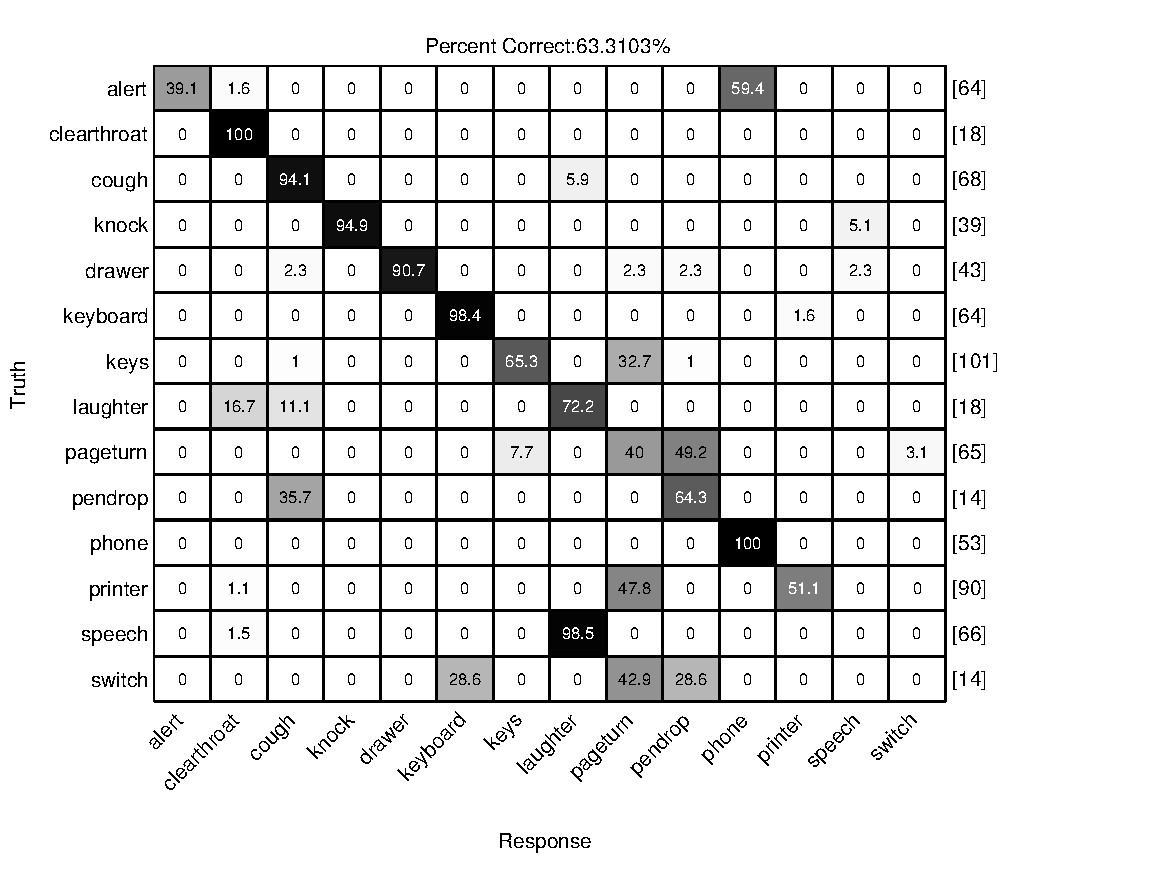
\includegraphics[width=\columnwidth]{confmatrix1-eps-converted-to.pdf}}
  \caption{Example of a figure with experimental results.}
  \label{fig:confmat_perfect}
\end{figure}

\begin{figure}[h]
  \centering
  \centerline{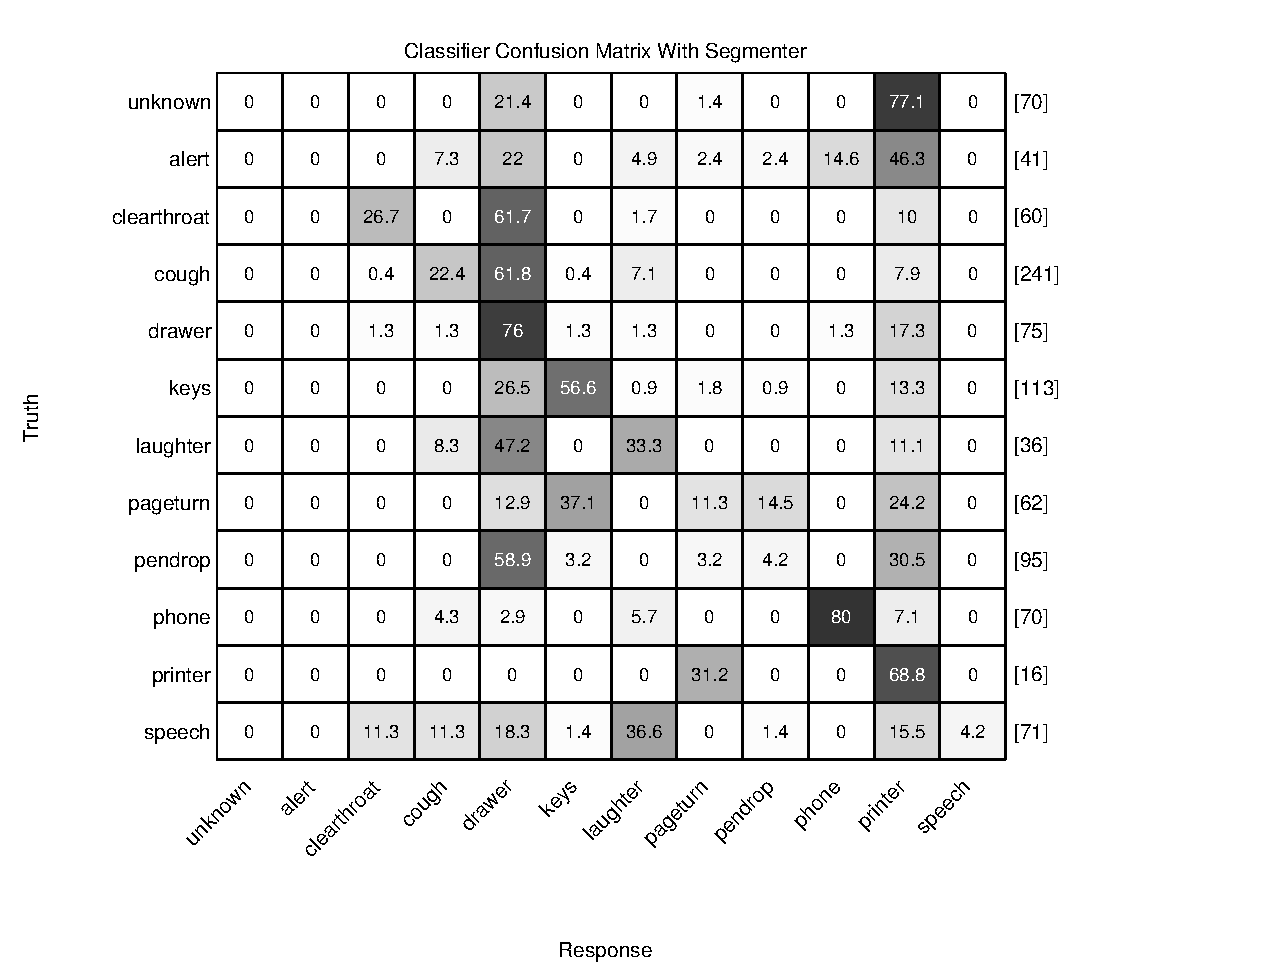
\includegraphics[width=\columnwidth]{confmatrix2-eps-converted-to.pdf}}
  \caption{Example of a figure with experimental results.}
  \label{fig:confmat_seg}
\end{figure}
